\chapter{Simulation der Systemkomponenten und Diskussion der Ergebnisse}
\label{cha:Diskussion}
Im folgenden Kapitel werden die Simulationsergebnisse vorgestellt. Zur Plausibilisierung der Daten werden die Modelle der Wasserstoffkomponenten im ersten Schritt mit in der Literatur angegebenen Messwerten abgeglichen. Im zweiten Schritt folgt die Präsentation der Simulationsergebnisse samt Berechnung der zur Bewertung herangezogenen Kennwerte. Dabei erfolgt zudem ein Vergleich der Systemkonzepte anhand der Bewertungskriterien.
 
\section{Validierung der Komponentenmodelle}
\label{sec:Sektion 1}
In der folgenden Validierung werden drei Systeme betrachtet: Einerseits ein alkalischer Elektrolyseur und eine PEM-Brennstoffzelle, weil diese beiden Bauarten in den Systemkonzepten genutzt werden. Andererseits ein PEM-Elektrolyseur, da diese Bauart, wie in \ref{subsec:Technologien der Wasserelektrolyse} angegeben, aufgrund von Vorteilen in der Dynamik der Last und bei der Baugröße aktuell an Relevanz zunehmen. 

\subsection{Komponenten der Systemkonzepte}
Zur Validierung des alkalischen Elektrolyseurs werden die von \citet{hammoudi_new_2012} dokumentierten Messwerte genutzt. Betrachtet wird eine Einzelzelle mit einer aktiven Zellfläche von $\SI{0,03}{\m\squared}$ deren Elektrodenabstand mit $\SI{5}{\milli\m}$ angenommen wird. Als Elektrolyt dient $30$-prozentige Kalilauge (daraus folgt $m=\SI{6,85}{\mol\per\l}$ \citep{periodensystem-online_dichtewerttabelle_nodate}). Betrieben wird die Zelle bei einem Druck von $\SI{1}{\bar}$ und es wird eine Temperatur von $30$ sowie $\SI{53,5}{\degreeCelsius}$ betrachtet.

\begin{figure}[h]
	\centering
		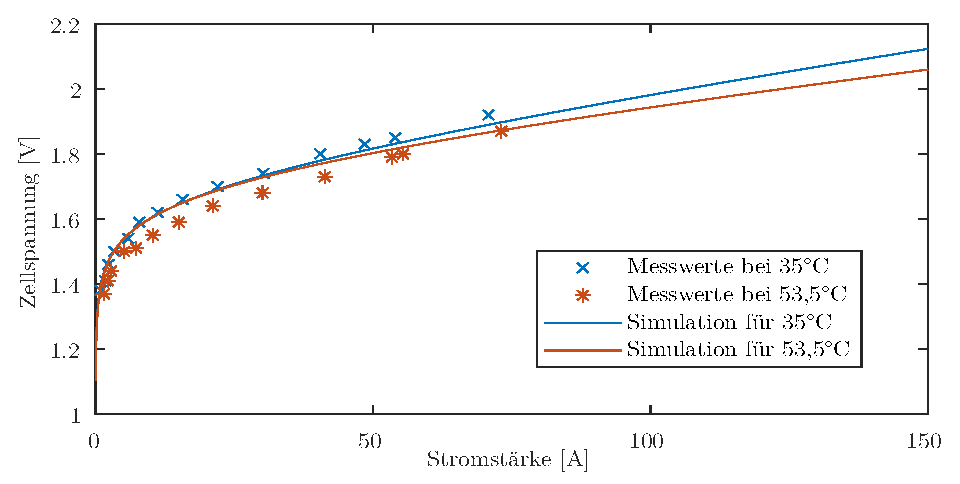
\includegraphics[scale=1]{Figures/ValidierungALK}
		\caption{Vergleich des Elektrolyseur-Modells mit Messwerten von \citet{hammoudi_new_2012}.}
\label{fig:ValALK}	
\end{figure}

Der von \citet{hammoudi_new_2012} dokumentierte Maximalwert der Stromstärke beträgt $\SI{73}{\A}$ und die minimale Teillast wird, wie in \ref{tb:VglElektrolyseur} angegeben, mit $\SI{20}{\%}$ des Maximalwerts angenommen. Somit kann als minimale Teillast des Elektrolyseurs im realen Betrieb von einer Stromstärke von $\SI{14,6}{\A}$ ausgegangen werden. In diesem Bereich beträgt der Fehler bei einer Temperatur von $\SI{35}{\degreeCelsius}$ maximal $\SI{1,6}{\%}$. Für eine Temperatur von $\SI{53,5}{\degreeCelsius}$ ergibt sich eine maximale Abweichung von $\SI{3,5}{\%}$ (Im Durchschnitt $\SI{2,2}{\%}$).\\
Es zeigt sich also, dass das Modell in der Lage ist, die Polarisationskurven alkalischer Elektrolyseure mit hinreichender Genauigkeit zu modellieren. Somit ist es für die Anwendung im Rahmen dieser Arbeit geeignet. Für folgende Arbeiten wird eine Validierung des Modells bei verschiedenen Druckniveaus empfohlen.\\

Um die Rechenzeit der Simulation gering zu halten wird in dieser Arbeit auf eine Simulation des thermischen Verhaltens der Elektrolysezelle verzichtet, allerdings kann diese bei Bedarf ohne weiteren Entwicklungsaufwand aus dem Brennstoffzellenmodell übernommen werden.
Eine weitere Möglichkeit zur Ausweitung des Modells sind dynamische Vorgänge, die in dieser Arbeit aufgrund der großen Zeitschritte der Simulation nicht beachtet wurden (Ausführlichere Begründung in \ref{subsec:Modellierung der Zelle}). Um diese zu berücksichtigen, kann die in der Energiebilanz (Gleichung \ref{gl:Energiebilanz}) enthaltene Instationarität der Zelltemperatur in der Modellierung des thermischen Verhaltens übernommen werden.\\

Zur Validierung der PEM-Brennstoffzelle werden Messwerte von \citet{chugh_experimental_2020} genutzt. Es handelt sich um einen Brennstoffzellenstack von 30 in Reihe geschalteten Einzelzellen. Die aktive Zellfläche einer Einzelzelle beträgt $\SI{0,005}{\m\squared}$ und die Dicke der Membran ist mit $\SI{50,8}{\micro\m}$ angegeben. Die betrachtete Betriebstemperatur beträgt $50$ und $\SI{80}{\degreeCelsius}$ und der Betriebsdruck bei $1$ und $\SI{2,5}{\bar}$.

\begin{figure}[h]
	\centering
		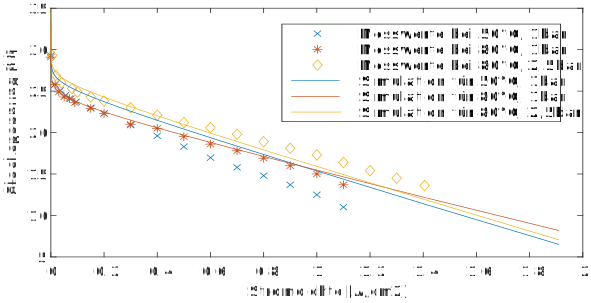
\includegraphics[scale=1]{Figures/ValidierungPEMFC}
		\caption{Vergleich des Brennstoffzellen-Modells mit Messwerten von \citet{chugh_experimental_2020}.}
\label{fig:ValPEMFC}	
\end{figure}

\citet{chugh_experimental_2020} dokumentieren einen Stromstärke von bis zu $\SI{1,4}{\A\per\cm\squared}$ und die minimale Teillast wird, wie in \ref{tb:VglBz} angegeben, für PEM-Zellen mit $\SI{10}{\%}$ des Maximalwerts angenommen. Daraus ergibt sich eine minimale Teillast von $\SI{0,14}{\A\per\cm\squared}$ für den realen Betrieb. Oberhalb des genannten Wertes liegt der Fehler bei einer Temperatur von $\SI{50}{\degreeCelsius}$ und einem Druck von $\SI{1}{\bar}$ zwischen $6,2$ und $\SI{30,6}{\%}$. Für $\SI{80}{\degreeCelsius}$ und $\SI{1}{\bar}$ ergeben sich Abweichungen von durchschnittlich $\SI{2,1}{\%}$ (Die maximale Abweichung beträgt $\SI{7,6}{\%}$). Wird der Druck auf $\SI{2,5}{\bar}$ angehoben, steigt der Fehler auf durchschnittlich $\SI{5,3}{\%}$ (Die maximale Abweichung beträgt in dem Fall $\SI{11,1}{\%}$).\\

Es zeigt sich somit, dass das Modell die Polarisationskurve von Brennstoffzellen bei hohen Betriebstemperaturen in einem akzeptablen Maß approximiert. Da die zur Simulation der Systemkonzepte eingesetzte Brennstoffzelle bei einer Betriebstemperatur von $\SI{80}{\degreeCelsius}$ betrieben wird, ist im Bezug auf die Modellierung der Brennstoffzelle von einer ausreichenden Genauigkeit auszugehen.\\
Die großen Abweichungen bei niedrigen Temperaturen lassen sich durch die Wahl des Durchtrittsfaktors ($\alpha$) und der Austauschstromdichte ($i_0$) begründen. Wie von \citet{falcao_review_2020} gezeigt, variieren die in der Literatur angegebenen Werte der beiden Parameter stark. So liegen die Angaben des Durchtrittfaktors zwischen $2$ und $0,5$ - die Angaben der Austauschstromdichte schwanken von $\SI{e-3}{}$ bis $\SI{e-9}{\A\per\cm\squared}$. Dabei werden teilweise getrennte Werte für Anode und Kathode angegeben, was aber auf die Größenordnung des Wertebereichs keinen Einfluss nimmt (Die angegebenen Wertebereiche beziehen sich auf die Anode, da dort höhere Verluste auftreten).\\
Es wird ersichtlich, dass die experimentell ermittelten Parameter einerseits von dem Aufbau des Modells abhängen, denn die Fitting-Parameter werden sowohl durch die Modellierung der anderen Verluste als auch durch im Modell nicht berücksichtigte weitere Faktoren beeinflusst. Andererseits spielt der Versuchsaufbau und die untersuchte Zelle eine gewichtige Rolle, da beispielsweise die Betriebstemperatur, der Betriebsdruck oder Materialeigenschaften die resultierenden Fitting-Parameter beeinflussen.
Einige Autoren nutzten daher Approximationen, um einen Temperatureinfluss auf den Durchtrittsfaktor oder die Austauschstromdichte im Modell zu berücksichtigen \citep{falcao_review_2020,milewski_modeling_2014}. Für die Modellierung von PEM-Zellen verspricht dies eine 
Steigerung der Genauigkeit bei niedrigen Temperaturen. Ob diese Maßnahme die Genauigkeit der Modellierung von alkalischen Zellen erhöht ist unklar, da die Validierungsergebnisse des alkalischen Elektrolyseurs keine signifikante Steigerung der Abweichungen bei zu- oder abnehmenden Temperaturen dokumentieren.\\
Eine weitere Möglichkeit zur Steigerung der Genauigkeit bei der Modellierung der Brennstoffzelle könnte die Beachtung der Konzentrationsüberspannungen sein. Denn diese treten insbesondere im oberen Lastbereich auf, und in diesem sind bei der Validierung zunehmende Abweichungen zu erkennen.\\

Die Validierung der Systemkomponenten ist somit im Hinblick auf die Genauigkeit der Simulationsergebnisse insgesamt als positiv zu bewerten: Die Elektrolysezelle wird über den abgebildeten Bereich zufriedenstellend modelliert. In dem für die Simulation relevanten Betriebspunkt trifft dies auch auf die Modellierung der PEM-Brennstoffzelle zu. Somit sind die in \ref{sec:Ergebnisse} präsentierten Simulationsergebnisse zur vorläufigen Bewertung der Systemkonzepte geeignet.
In Zukunft sollte darüber hinaus eine Validierung der Modellierung des thermischen Verhaltens erfolgen.

\subsection{PEM-Elektrolyseur}
Die Daten zur Validierung der PEM-Elektrolysezelle sind \citet[S. 36]{tjarks_pem-elektrolyse-systeme_2017} entnommen. Betrachtet wird eine Einzelzelle mit einer aktiven Zellfläche von $\SI{0,0025}{\m\squared}$ deren Membran mit einer Dicke von $\SI{150}{\micro\m}$ abgeschätzt wird (vergleiche \citet{rashid_hydrogen_2015}).
Es werden Betriebstemperaturen von $30$, $60$ und $\SI{80}{\degreeCelsius}$ bei einem Druck von $\SI{1}{\bar}$ untersucht.\\

\begin{figure}[h]
	\centering
		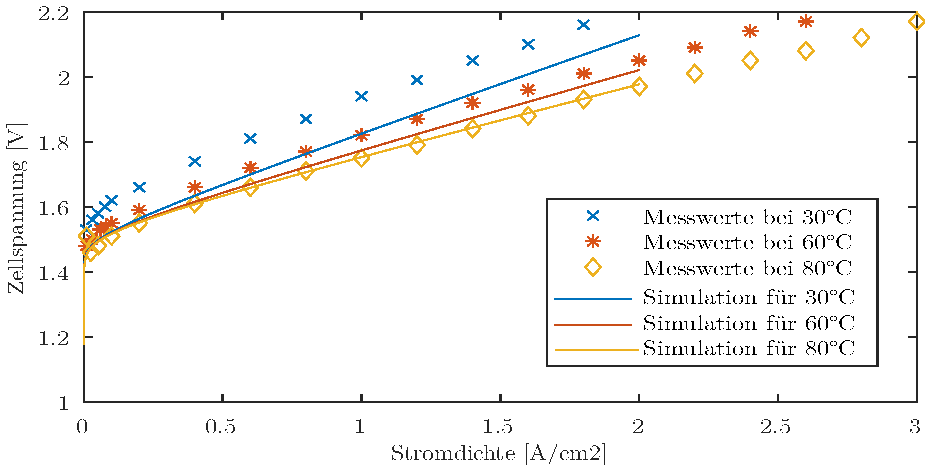
\includegraphics[scale=1]{Figures/ValidierungPEMEC}
		\caption{Vergleich des Elektrolyseur-Modells mit Messwerten von \citet{tjarks_pem-elektrolyse-systeme_2017}.}
\label{fig:ValPEMEC}	
\end{figure}

Die folgenden Angaben beziehen sich auf Stromdichten oberhalb von $\SI{0,2}{\A\per\cm\squared}$, da die minimale Teillast nach Tabelle \ref{tb:VglBz} für PEM-Zellen mit $\SI{10}{\%}$ der Maximalen Stromdichte angenommen wird. Bei einer Temperatur von $\SI{30}{\degreeCelsius}$ ergeben sich Abweichungen von  $\SI{22,3}{\%}$ bei der minimalen Teillast und $\SI{4,4}{\%}$ bei Maximallast. 
Für eine Temperatur von  $\SI{60}{\degreeCelsius}$ liegt der Fehler über den gesamten Leistungsbereich unter $\SI{2,9}{\%}$, für $\SI{80}{\degreeCelsius}$ unterhalb von $\SI{0,5}{\%}$.\\

Es zeigt sich somit auch für den PEM-Elektrolyseur, dass das Modell im oberen Temperaturbereich in der Lage ist, die Polarisationskurve ausreichend genau abzubilden. Wie auch bei der PEM-Brennstoffzelle liegen bei niedrigen Temperaturen signifikante Abweichungen zu den Messwerten vor. Im Gegensatz zur Brennstoffzelle nehmen diese aber nicht bei hohen, sondern bei niedrigen Lasten zu. Außerdem zeigt ein Vergleich der Messwerte des PEM-Elektrolyseurs und der PEM-Brennstoffzelle, dass sich der Temperatureinfluss auf die Zellspannung in den beiden Fällen deutlich unterscheidet:\\ 
Im Falle der Brennstoffzelle (Abbildung \ref{fig:ValPEMFC}) zeigt sich eine gesteigerte Temperatur erst im oberen Lastbereich, wohingegen sich die Zellspannung bei $0,2$ bis $\SI{0,3}{\A\per\cm\squared}$ trotz einen Temperaturdifferenz von $\SI{30}{\degreeCelsius}$ nicht signifikant unterscheidet.\\
Im Falle des Elektrolyseurs (Abbildung \ref{fig:ValPEMEC}) ist schon im unteren Lastbereich ein signifikanter Unterschied der Zellspannung für die abgebildeten Temperaturen sichtbar, der mit zunehmender Stromdichte linear ansteigt.\\

Daraus lässt sich schlussfolgern, dass für den gewählten Elektrolyseur und die Brennstoffzelle eine einheitliche Parametrierung insbesondere über einen größeren Temperaturbereich keine zufriedenstellenden Ergebnisse liefern kann. Ob diese Beobachtung allgemein auf den Vergleich von Elektrolyseuren und Brennstoffzellen anzuwenden ist, bleibt allerdings unklar. In folgenden Arbeiten sollte daher untersucht werden, ob weitere Messreihen den unterschiedlichen Temperatureinfluss auf die Polarisationskurven bestätigen. Dies würde im Modell gegebenenfalls eine getrennte Parametrierung von Brennstoffzellen und Elektrolyseuren erfordern.\\

\section{Ergebnisse der Simulationen der Systemkonzepte}
\label{sec:Ergebnisse}
Die Simulationen wurden mit Zeitschritten von $\SI{900}{\s}$ ($=\SI{15}{\minute}$) durchgeführt. Es wurde der Dymola-Standard-Löser \textit{Dassl} mit einer Toleranz von $\SI{e-4}{}$ verwendet.
Als Ergebnisse der Simulation sind drei Kennwerte von Bedeutung: Der jährliche Strombedarf, die Stromeinspeisungen und die Gaseinsparungen. Im folgenden werden die Kennwerte des aktuellen Systems sowie der entwickelten Systemkonzepte präsentiert. Die Stromeinsparungen sind in Abbildung \ref{fig:Strom} graphisch wiedergegeben, in Tabelle \ref{tb:ErgebnisseSim} sind die Kennwerte für die 4 Konzepte aufgelistet. Für eine genauere Evaluierung der Konzepte sollten in Zukunft Simulationen mit Messreihen des Prozessgasverbrauchs durchgeführt werden, da der benötigte Stoffmengenstrom einen großen Einfluss auf die Effizienz des Elektrolyseurs und der Brennstoffzelle hat und die Ergebnisse somit maßgeblich beeinflusst.\\
 
Für das aktuelle System wird ein Jahres-Strombedarf von $\SI{959,3}{\megaWh}$ für den an 2018 angelehnten Prozessgasbedarf prognostiziert, mit den Daten für 2019 ergibt sich ein Strombedarf von $\SI{915,173}{\megaWh}$.

\paragraph{Konzept 1}\ \\
Die Verwendung einer Brennstoffzelle zur Nutzung des Wasserstoffüberschusses führt zu Stromeinsparungen von $12,9$ beziehungsweise $\SI{5,9}{\megaWh}$ pro Jahr im Vergleich zum aktuellen System. Bei alleiniger Verwendung der Brennstoffzelle wird kein Strom ins Netz eingespeist. Dies entspricht den Erwartungen, weil die Ausgangsleistung der Brennstoffzelle aufgrund der Umwandlungsverluste stets kleiner als die Eingangsleistung des Elektrolyseurs ist. Die Gaseinsparungen betragen $\SI{14,1}{\megaWh}$ für den Prozessgasverbrauch nach den 2018er Daten, für die 2019er Daten ergeben sich $\SI{6,6}{\megaWh}$.
\paragraph{Konzept 2}\ \\
Bei Installation einer PV-Anlage ergeben sich Stromeinsparungen von $\SI{66,3}{\megaWh}$ für beide Verläufe des Prozessgasbedarfs. 
Die berechnete Einspeisung bei Verwendung einer PV-Anlage beträgt unabhängig vom sonstigen Systemaufbau und dem Prozessgasverbrauch $\SI{4,3}{\megaWh}$. Dies lässt darauf schließen, dass die Stromeinspeisung außerhalb der Arbeitszeit, also beispielsweise in den Abendstunden oder am Wochenende, auftritt.

\paragraph{Konzept 3}\ \\
Wird das System um eine PV-Anlag und eine Brennstoffzelle erweitert ergeben sich jährliche Stromeinsparungen von $84,7$ beziehungsweise $\SI{75,0}{\megaWh}$. Die Gaseinsparungen liegen bei $13$ beziehungsweise $\SI{6,5}{\megaWh}$.\\

Ein Vergleich der Konzepte 1 bis 3 zeigt, dass sich die PV-Anlage und die Brennstoffzelle nicht gegenseitig beeinflussen: Die Abweichungen einer Berechnung der Endwerte von Konzept 3 als Addition von Konzept 1 und 2 liegen im Verhältnis zu den Simulationsergebnissen für die Stromeinsparungen unter $\SI{0,6}{\%}$ und für die Gaseinsparung unter $\SI{1,4}{\%}$ (Eine Erklärung für die Abweichungen ist die gewählte Toleranz der Simulation). Dieses Verhalten liegt darin begründet, dass die maximale elektrische Leistung der Brennstoffzelle ($\SI{24,475}{\kiloW}$) und der PV-Anlage ($\SI{79,980}{\kiloW}$) in Summe kleiner ist als der Strombedarf während der Arbeitszeit (über $\SI{200}{\kiloW}$). Somit kommt es während beide Komponenten im Betrieb sind zu keinem Zeitpunkt zu einem Überangebot von erzeugtem Strom, welches ins Netz eingespeist wird. Aus diesem Grund führt die Verwendung beider Komponenten im Vergleich zur Einzel-Betrachtung nicht zu einer Steigerung der Einspeisung oder einer Verminderung der Einsparungen beim Strombedarf.

\paragraph{Konzept 4}\ \\
Die Simulationsergebnisse bei einer Verwendung einer PV-Anlage in Kombination mit einem Gasspeicher weisen keine signifikanten Unterschiede zu den Ergebnissen ohne Gasspeicher auf. Aus den Simulationsergebnissen geht hervor, dass der Speicher bei der gewählten Betriebsstrategie stets mit weniger als $\SI{e-14}{\kg}$ befüllt ist und keine Senkung der Stromeinspeisung ins Netz zu verzeichnen ist. Wie bereits festgestellt besteht der Überschuss von PV-Strom außerhalb der Betriebszeiten. Aus der geringen Beladung des Speichers lässt sich daher schließen, dass die überschüssige Leistung stets geringer ist als die benötigte Leistung bei der minimalen Teillast des Elektrolyseurs und daher keine Einspeicherung des Stromüberschusses in Form von Prozessgasen möglich ist.\\
Somit bringt die Verwendung des Gasspeichers im Energiesystem keinen Nutzten und findet bei der Berechnung der Kapitalwerte und der \ce{CO2}-Emissionen keine Berücksichtigung.\\

Eine alternative Betriebsstrategie bei Wasserstoffsystemen mit Gasspeichern ist nach \citet{bocklisch_optimierendes_2010} die Nutzung des Gasspeichern als Puffer zur Verminderung der dynamischen Beanspruchung des Elektrolyseurs. Als Vorteil gibt er einerseits eine Effizienzsteigerung an, weil im dynamischen Betrieb zusätzliche Verluste auftreten. Andererseits führt er an, dass dynamische Beanspruchung zur Degradation der Zellleistung beiträgt und die Lebensdauer der Zelle senkt.\\



\begin{figure}[h]
	\centering
		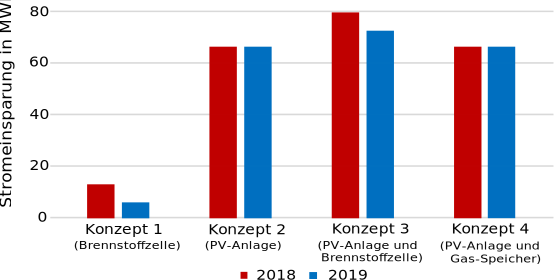
\includegraphics[scale=1]{Figures/Stromverbrauch_Sim_2}
		\caption{Vergleich der Simulationsergebnisse für den Jahresstromverbrauch des aktuellen Systems und der Konzepte samt Angabe der Stromeinsparungen im Vergleich zum aktuellen System.}
\label{fig:Strom}	
\end{figure}

\begin{table}[htb]
		\centering
		\caption{Vergleich der Stromeinsparungen, Einspeisung und Gaseinsparung der Systemkonzepte (Im erste Block sind die Daten für die Bedarfsverläufe aus 2018 und im zweite die Daten für die Bedarfsverläufe aus 2019 angegeben).}
		\begin{tabular}{l c c c}
		\toprule 
		& Stromeinsparungen & Einspeisung & Gaseinsparung
		\\
	    & in MWh & in MWh & in MWh\\
		\midrule
		Konzept 1 & $12,857$ &    -    & $14,083$\\
		Konzept 2 & $66,296$ & $4,313$ &    -    \\
		Konzept 3 & $79,637$ & $4,313$ & $14,032$\\
		Konzept 4 & $66,296$ & $4,313$ &    -    \\
		\midrule
		Konzept 1 & $5,858$  &    -    & $6,620$\\
		Konzept 2 & $66,295$ & $4,313$ &    -   \\
		Konzept 3 & $72,489$ & $4,313$ & $6,526$\\
		Konzept 4 & $66,295$ & $4,313$ &    -   \\
		\bottomrule
		\end{tabular}
		\label{tb:ErgebnisseSim}
\end{table}	
\FloatBarrier

\paragraph{Kapitalwerte der Systemkonzepte}\ \\
Die Kapitalwerte werden mithilfe der in \ref{Apx:Kapitalwert} angegebenen Parameter berechnet. In Abbildung \ref{fig:Kapitalwerte} werden die Kapitalwerte der Systemkonzepte graphisch gegenübergestellt, in Tabelle \ref{tb:Kapitalwerte} sind die Investitionskosten sowie jährliche Einnahmen und Ausgaben angegeben.\\

Für die Investition in eine Brennstoffzelle ergibt sich ein Kapitalwert von $5.\SI{847}{\sieuro}$ für den an 2018 angelehnten Prozessgasbedarf, mit den Daten für 2019 ergibt sich ein Kapitalwert von $-15.\SI{338}{\sieuro}$. Die Investition ist somit anhand des Kapitalwerts als tendenziell negativ zu bewerten. Um die Aussagekraft der Bewertung zu erhöhen, ist es sinnvoll, die Wahrscheinlichkeiten der beiden simulierten Szenarien abzuschätzen und dies in die Bewertung mit einfließen zu lassen. Für den Fall, dass in Zukunft mit steigendem Wasserstoffüberschuss zu rechnen ist, könnte sich die Investition in eine Brennstoffzelle als wirtschaftlich sinnvoll herausstellen.\\

Einen verbesserten Ansatz könnte die Installation einer Brennstoffzelle mit einer kleineren Zellfläche in Kombination mit einem Wasserstoffspeicher darstellen. Dadurch kann bei einer nahezu gleichbleibenden Stromeinsparung eine deutliche Verminderung der Investitionskosten erreicht werden, was durch eine überschlägige Berechnung verdeutlicht werden soll:\\
Bei den betrachteten Verläufen des Prozessgasbedarfs beträgt der maximal denkbare Überschuss an Wasserstoff ungefähr $\SI{5,3}{\kg}$ (In maximal $\SI{2}{\hour},\SI{45}{\minute}$ pro Tag wird überschüssiger Wasserstoff produziert und der maximale Stoffmengenstrom beträgt $\SI{0,2643}{\mol\per\s}$). Wird die Umwandlung des Wasserstoffs  nicht zeitgleich, sondern über den Tag verteilt vollzogen, reichen  $\frac{\SI{2}{\hour},\SI{45}{\minute}}{\SI{24}{\hour}} =  \SI{11,5}{\%}$ der im aktuellen Konzept veranschlagten Maximalleistung aus, um den Wasserstoffüberschuss vollständig zu nutzen. Dadurch sinken die Investitionskosten der Brennstoffzelle auf $5.\SI{250}{\sieuro}$ (siehe \ref{Apx:Kapitalwert}). Investitonskosten in einen Wasserstoffspeicher können, wie in \ref{Apx:Kapitalwert} angegeben, mit $\SI{594}{\sieuro\per\kg_{H2}}$ abgeschätzt werden. Somit ergeben sich Gesamt-Investitionskosten von $\SI{8.400}{\sieuro}$, was einem Viertel der Investitionskosten des simulierten 
Brennstoffzellen-Konzepts entspricht. Da durch den zusätzlichen Betrieb des Speichers mit steigenden Betriebskosten und zusätzlichem Stromverbrauch zu rechnen ist, soll an dieser Stelle auf eine Berechnung des Kapitalwerts verzichtet werden. Allerdings zeigt die Abschätzung, dass durch die Kombination mit einem Gasspeicher mit einer deutliche Verbesserung hinsichtlich des Kapitalwerts zu rechnen ist.\\

Die Investition in eine PV-Anlage ergibt unabhängig vom verwendeten Bedarfsverlauf einen Kapitalwert von $84.\SI{726}{\sieuro}$. Die Bewertung der Wirtschaftlichkeit der Investition anhand des Kapitalwerts fällt also positiv aus.\\ 

Dies trifft auch auf die Kombination aus PV-Anlage und Brennstoffzelle zu, für die sich Kapitalwerte von $91.\SI{824}{\sieuro}$ und $70.\SI{220}{\sieuro}$ ergeben.
Es ist aber zu beachten, dass verglichen mit Konzept 2 die Mehrinvestition in eine Brennstoffzelle gemessen am Kapitalwert keinen deutlichen Mehrwert mit sich bringt. So erhöht sich der Kapitalwert für das Szenario 2018 bezogen auf die gesteigerten Investitionskosten nur unwesentlich und im Szenario 2019 sinkt der Kapitalwert durch die Mehrinvestition in eine Brennstoffzelle.\\

Zusammenfassend lässt sich daher sagen, dass nach Aussage des Kapitalwerts die Investition in eine PV-Anlage lohnenswert ist. Die ökonomische Bewertung der Brennstoffzelle hängt von dem prognostizierten Prozessgasverbrauch ab, fällt aber tendenziell negativ aus. Optimierungen des Brennstoffzellen-Konzepts versprechen aber deutliche Verbesserungen im Hinblick auf die ökonomische Bewertung.

\begin{figure}[h]
	\centering
		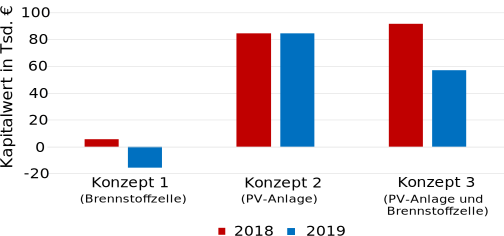
\includegraphics[scale=1]{Figures/Kapitalwerte}
		\caption{Kapitalwerte der Systemkonzepte.}
\label{fig:Kapitalwerte}	
\end{figure}

\begin{table}[htb]
		\centering
		\caption{Kapitalwerte der Konzepte sowie Kosten, die in die Berechnung einfließen (Im erste Block sind die Daten für die Bedarfsverläufe aus 2018 und im zweite die Daten für die Bedarfsverläufe aus 2019 angegeben).}
		\begin{tabular}{l c c c c}
		\toprule
		 & Investitionskosten & Einnahmen & Ausgaben & Kapitalwert\\
		& in € & in € & in € & in €\\
		Formelzeichen & $I_0$ & $Z_{ein}$ & $Z_{aus}$ & C\\
		\midrule
		Konzept 1 & $ 33.286$ & $ 3.550,63$ & $  259,71$ & $ 5.846,72$\\
		Konzept 2 & $ 80.352$ & $15.087,43$ & $1.205,00$ & $84.725,62$\\
		Konzept 3 & $113.638$ & $18.743,31$ & $1.464,71$ & $91.823,88$\\
		\midrule
		Konzept 1 & $ 33.286$ & $ 1.627,71$ & $  118,33$ & $-15.337,78$\\
		Konzept 2 & $ 80.352$ & $15.087,43$ & $1.205,00$ & $ 84.725,62$\\
		Konzept 3 & $113.638$ & $16.785,12$ & $1.323,33$ & $ 70.219,98$\\
		\bottomrule
		\end{tabular}
		\label{tb:Kapitalwerte}
\end{table}	

\FloatBarrier

\paragraph{CO2-Einsparungen der Systemkonzepte}\ \\
Die benötigten Parameter zur Berechnung der \ce{CO2}-Einsparungen sowie ihre Herleitung sind in \ref{Apx:CO2} aufgelistet. In Abbildung \ref{fig:CO2Einsparungen} werden die Einsparungen graphisch gegenübergestellt, die Bestandteile der Berechnung sind in Tabelle \ref{tb:CO2Einsparungen} aufgelistet.\\

Für die Verwendung einer Brennstoffzelle ergeben sich \ce{CO2}-Einsparungen von $\SI{8,0}{\tonne}$ für den an 2018 angelehnten Prozessgasbedarf, mit den Daten von 2019 werden $\SI{3,6}{\tonne}$ \ce{CO2} eingespart. Die Verwendung einer PV-Anlage im Energiesystem führt zu \ce{CO2}-Einsparungen von $\SI{24,8}{\tonne}$, bei einer Kombination von PV-Anlage und Brennstoffzelle liegen die \ce{CO2}-Einsparungen bei $\SI{32,9}{\tonne}$ beziehungsweise bei $\SI{28,5}{\tonne}$.\\

Alle drei Systemkonzepte versprechen somit eine Senkung der jährlichen \ce{CO2}-Emissionen. Die Einsparungen bei Verwendung der PV-Anlage sind dabei je nach Szenario $\SI{310}{\%}$ beziehungsweise $\SI{680}{\%}$ höher als die Einsparungen bei Verwendung einer Brennstoffzelle. 


\begin{figure}[h]
	\centering
		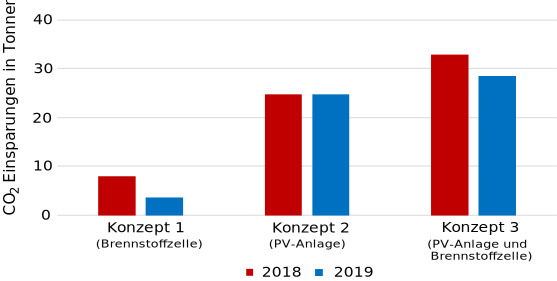
\includegraphics[scale=1]{Figures/CO2Einsparungen}
		\caption{ \ce{CO2}-Einsparungen der Systemkonzepte.}
\label{fig:CO2Einsparungen}	
\end{figure}

\begin{table}[htb]
		\centering
		\caption{\ce{CO2}-Einsparungen der Systemkonzepte sowie Einsparungen elektrischer Energie, Gaseinsparungen und bei der Produktion der Komponenten entstehende \ce{CO2}-Emissionen (Im erste Block sind die Daten für die Bedarfsverläufe aus 2018 und im zweite die Daten für die Bedarfsverläufe aus 2019 angegeben).}
		\begin{tabular}{l c c c c}
		\toprule
		 & Eisp. el. Energie & Gaseinsp. & \ce{CO2}-Em. der Prod. & \ce{CO2}-Einsp. \\
		& in MWh & in MWh & in Tonnen & in Tonnen\\
		Formelzeichen & $\Delta P_{el}$ & $\Delta Q$ & $\Delta m_{Prod.}$ & $\Delta m_{\ce{CO2}}$\\
		\midrule
		Konzept 1 & $12,957$ & $14,083$ & $0,038$ & $ 7,992$\\
		Konzept 2 & $70,609$ &    -     & $3,530$ & $24,784$\\
		Konzept 3 & $83,950$ & $14,032$ & $3,568$ & $32,919$\\
		\midrule
		Konzept 1 & $ 5,858$ & $6,620$ & $0,756$ & $ 3,643$\\
		Konzept 2 & $70,609$ &    -    & $3,530$ & $24,784$\\
		Konzept 3 & $76,802$ & $6,526$ & $3,568$ & $28,542$\\
		\bottomrule
		\end{tabular}
		\label{tb:CO2Einsparungen}
\end{table}

